\section{Tools}

    This section contains a brief overview of tools used for purposes not
    directly related to programming.

\subsection{Git and GitHub}
\label{subsec:git}
    Any software of a certain size needs source control management (SCM). Git is
    one of the most popular SCM systems today, and one that all team members had
    some experience with. Therefore Git was an obvious choice for this project.

    GitHub \cite{github, githubPage} is an online service offering hosting and a web interface to Git, and is
    probably the most popular code repository for open source projects. Because of
    its popularity, and because the team members have all had previous experience
    with GitHub, we decided to make it our central code repository.

\begin{figure}[htb]
  \centering
  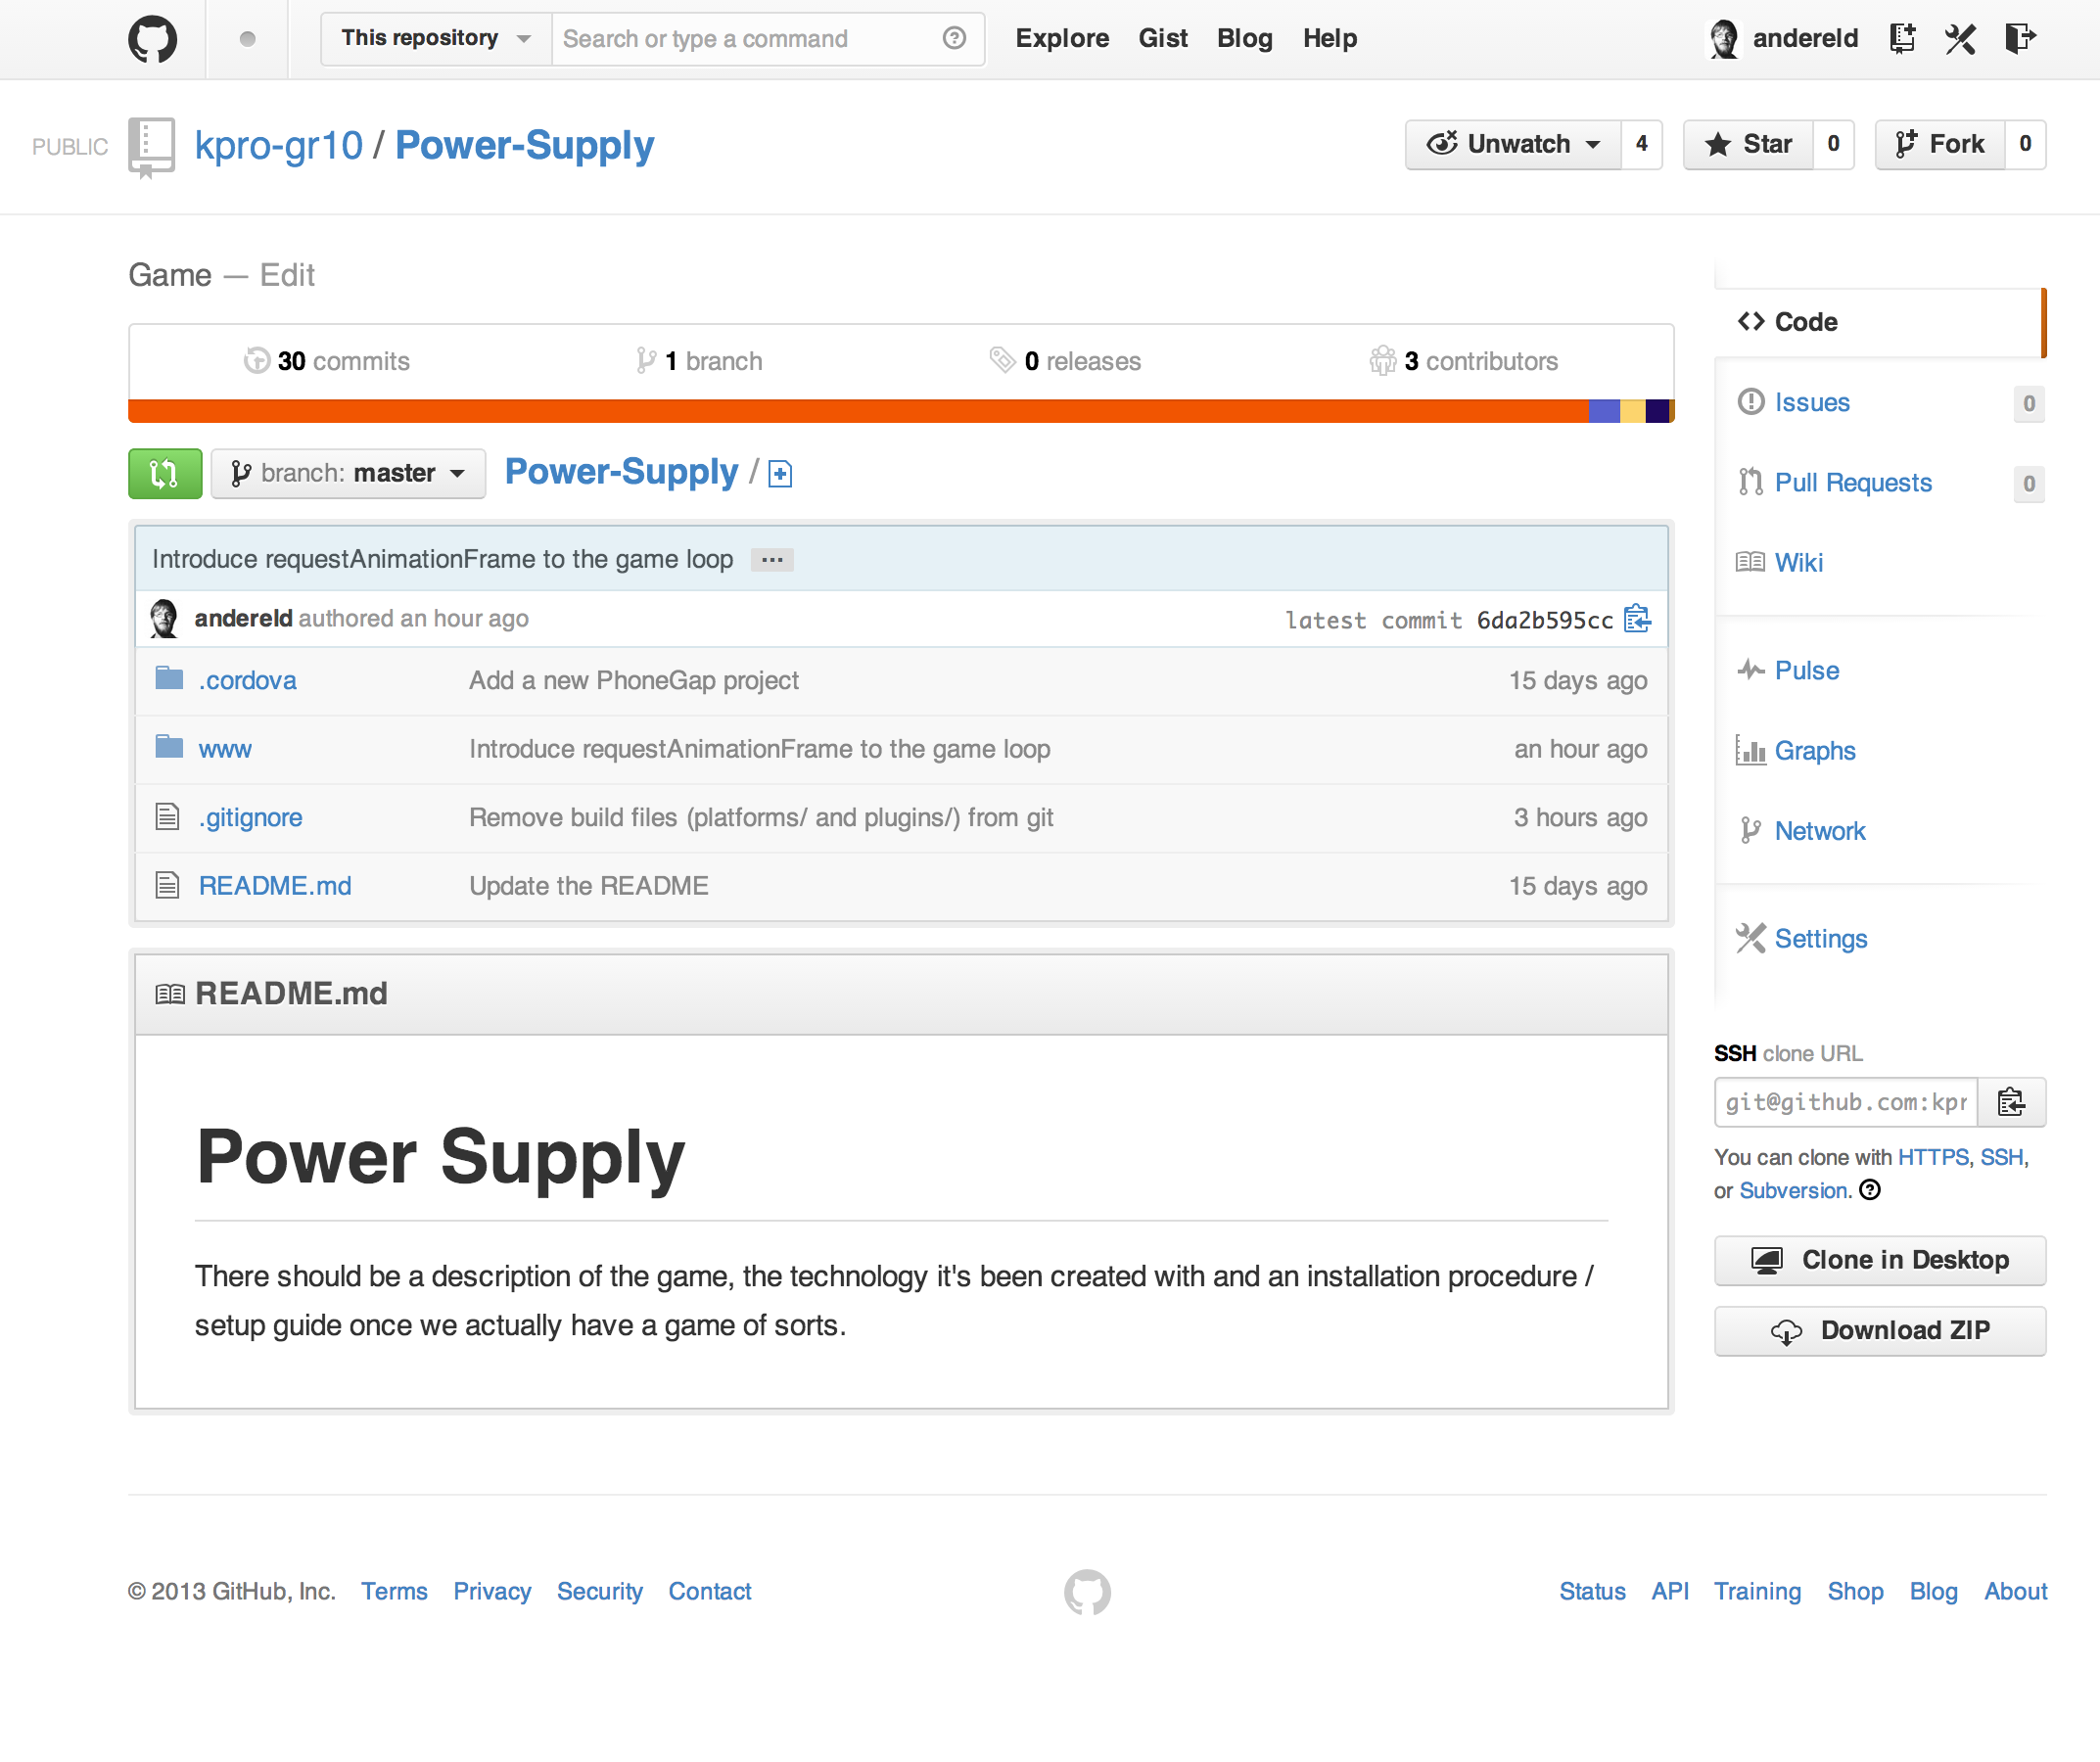
\includegraphics[width=1\textwidth]{pictures/github.png}
  \caption{GitHub project page}
\end{figure}

\subsection{AgileZen}
    As we've chosen the Scrum methodology, a Scrum board of sorts was necessary to
    keep track of our activities. \href{https://github.com}{GitHub} has a
    feature called ``Issues'' which allows a project to keep a list of unfinished
    tasks tagged with different labels, e.g. the traditional ``To Do'', ``In
    Progress'' etc. While this would work, we prefer a solution more similar to an
    actual whiteboard. \cite{agileZen}

    \begin{figure}[htb]
      \centering
      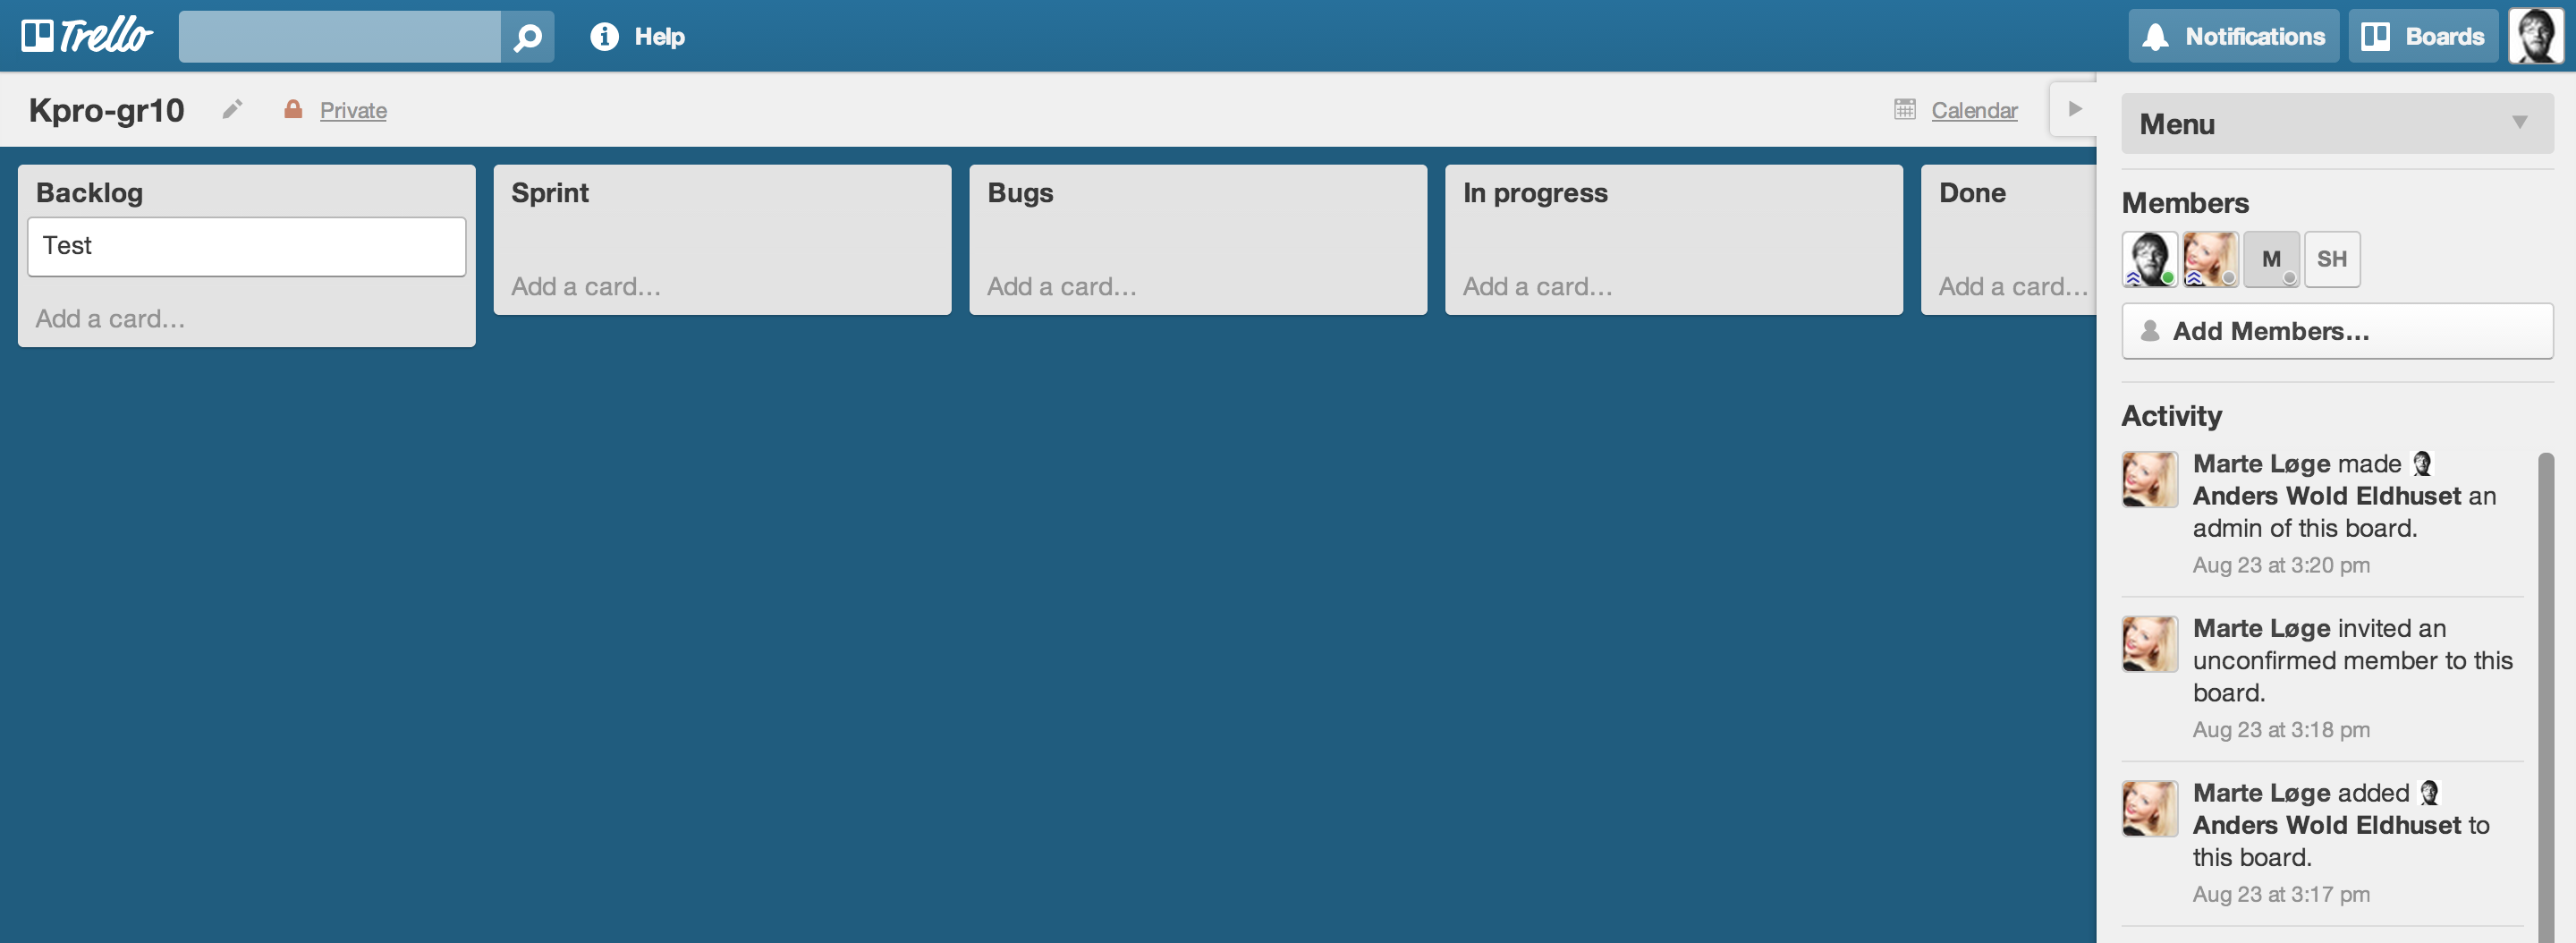
\includegraphics[width=1\textwidth]{pictures/trello.png}
      \caption{Trello Scrum board}
    \end{figure}

    One such solution is \href{https://trello.com}{Trello} \cite{trello, trelloPage}, an online Scrum
    board application. While Trello would work nicely, and was what we initially
    decided on using, one of the team members had used a competing product called
    \href{http://www.agilezen.com/}{AgileZen}. AgileZen has a few more features,
    such as sprint statistics, and we decided on using that instead of Trello.
    While AgileZen is normally a paid service, we managed to negotiate a free
    project account as an open source project.

    \begin{figure}[htb]
      \centering
      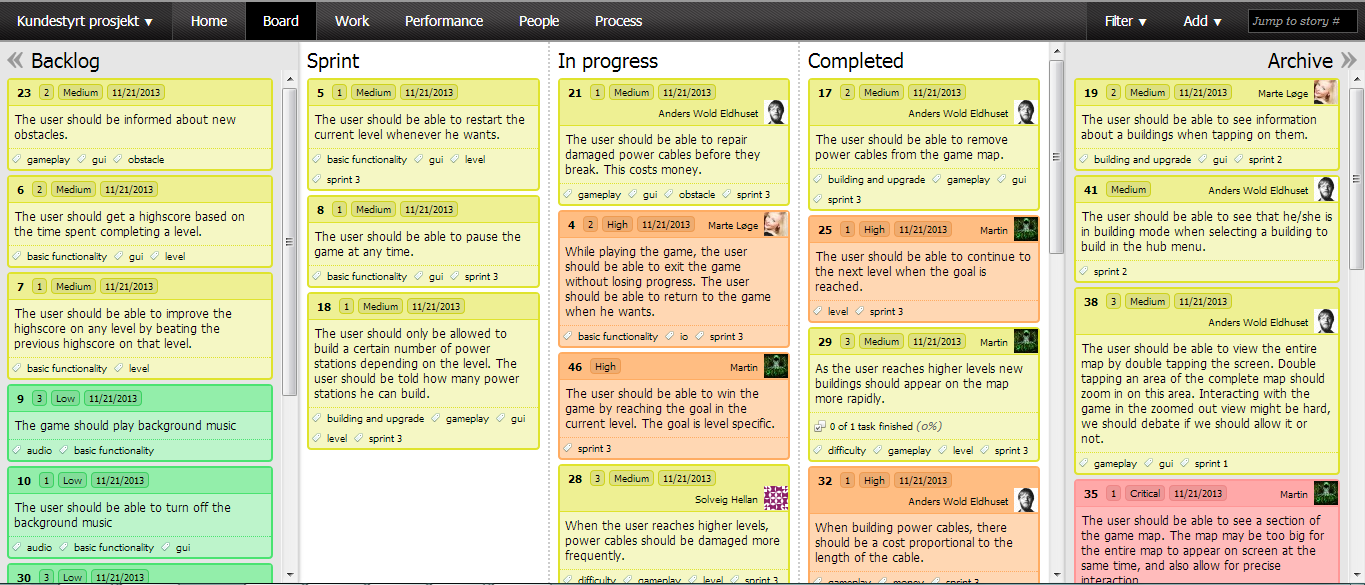
\includegraphics[width=1\textwidth]{pictures/agilezen2.png}
      \caption{AgileZen Scrum board}
    \end{figure}

\subsection{Google Drive}
    There are quite a few documents and spreadsheets to write in the course
    of a project such as this, and a collaborative text editing system
    makes it much easier to produce these. For this purpose we chose to use
    \href{https://drive.google.com}{Google Docs} (part of the Google Drive
    service). Google Docs was an obvious choice because of its popularity and
    reliability, and because all of the team members were already familiar with the
    service. \cite{drive}

    \begin{figure}[htb]
      \centering
      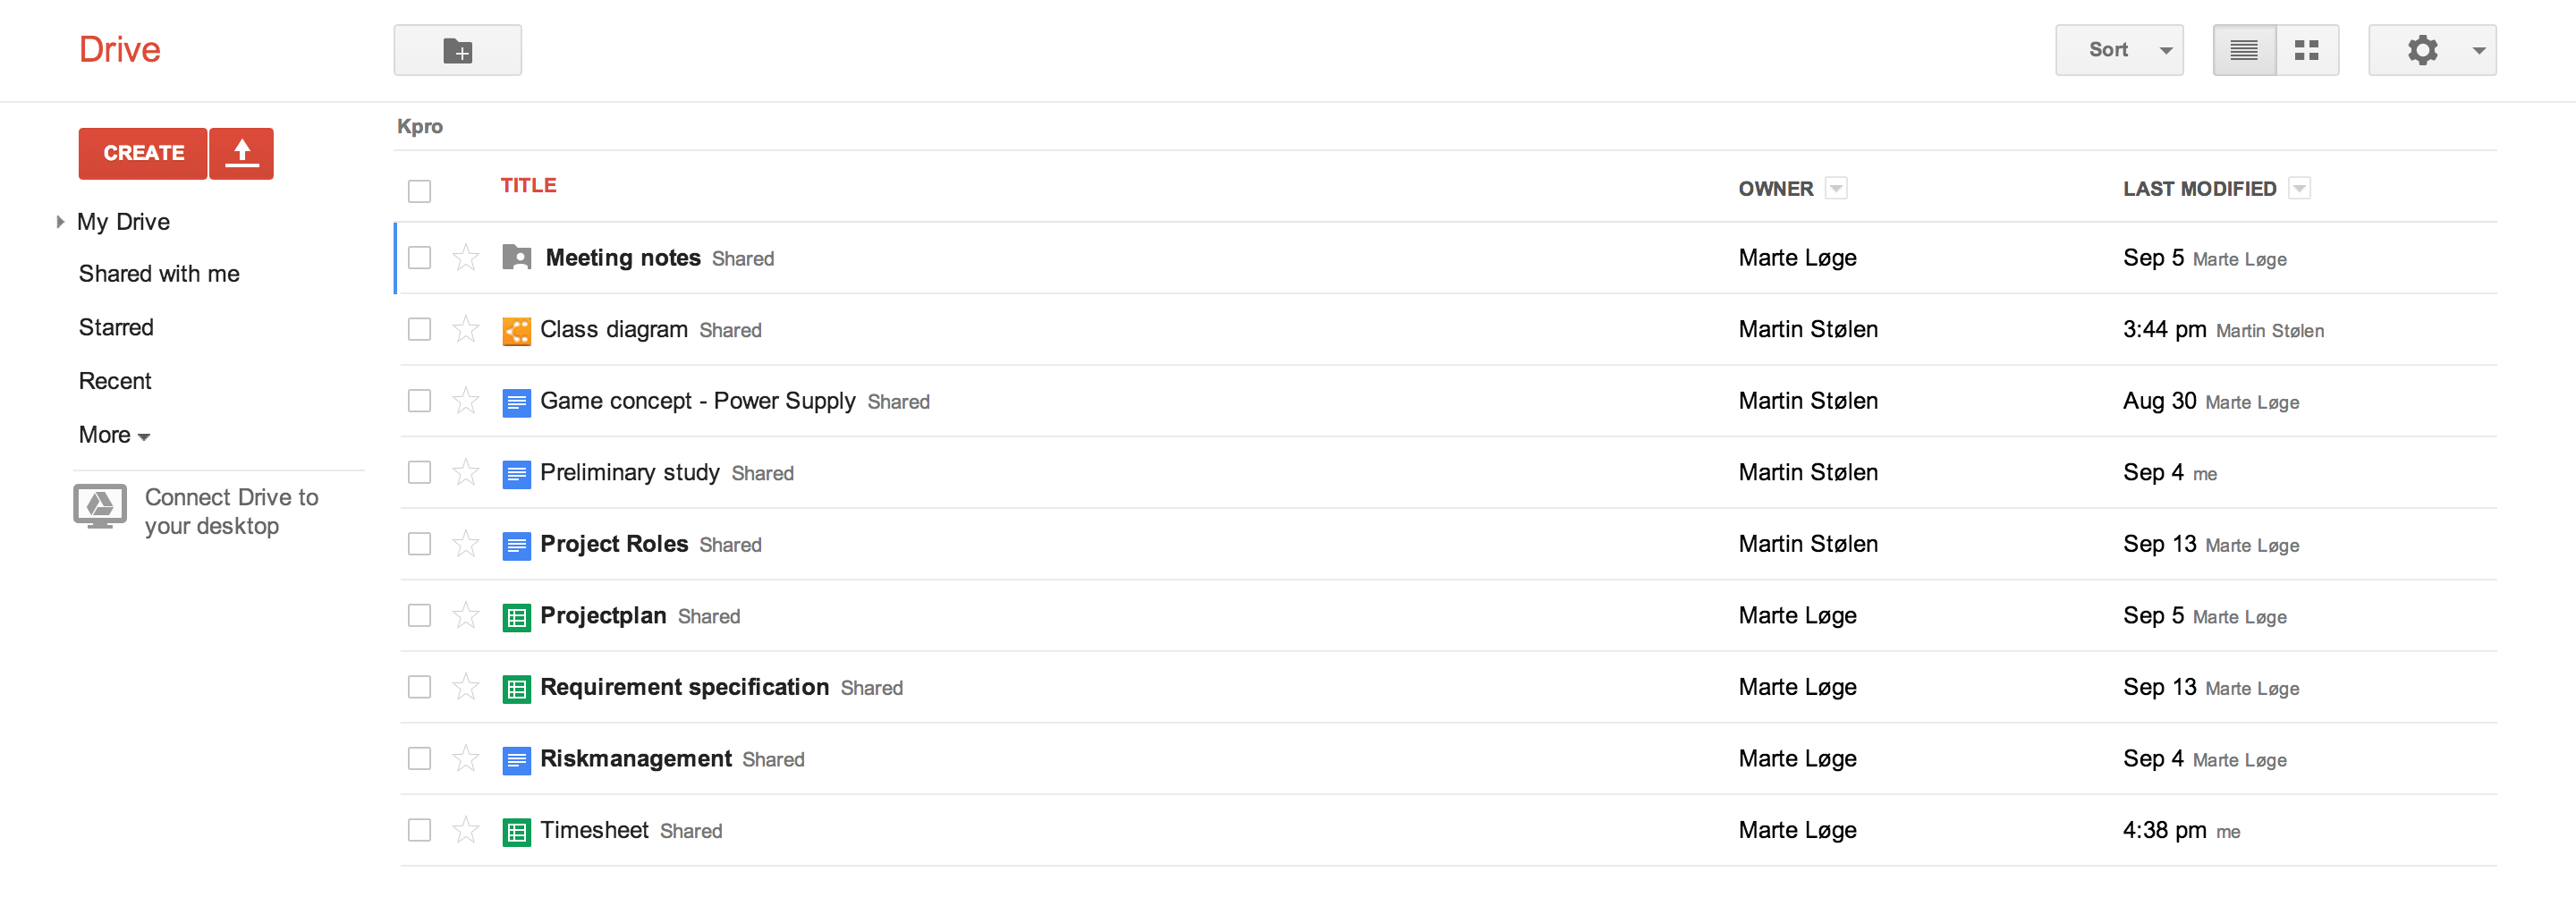
\includegraphics[width=1\textwidth]{pictures/google_drive.png}
      \caption{A shared Google Drive directory}
    \end{figure}

\subsection{Dropbox}
    While Google Drive works well for collaborating on text documents and
    spreadsheets, it is arguably not an ideal service for arbitrary file
    sharing. Because there was a need to share images and other binary files, we
    supplemented Google Drive with \href{https://www.dropbox.com/}{Dropbox}. Like
    Google Drive, Dropbox is a very popular and proven service, and one that all of
    the team members were already familiar with. It was therefore a sensible choice
    for our purposes. \cite{dropbox}

    \begin{figure}[htb]
      \centering
      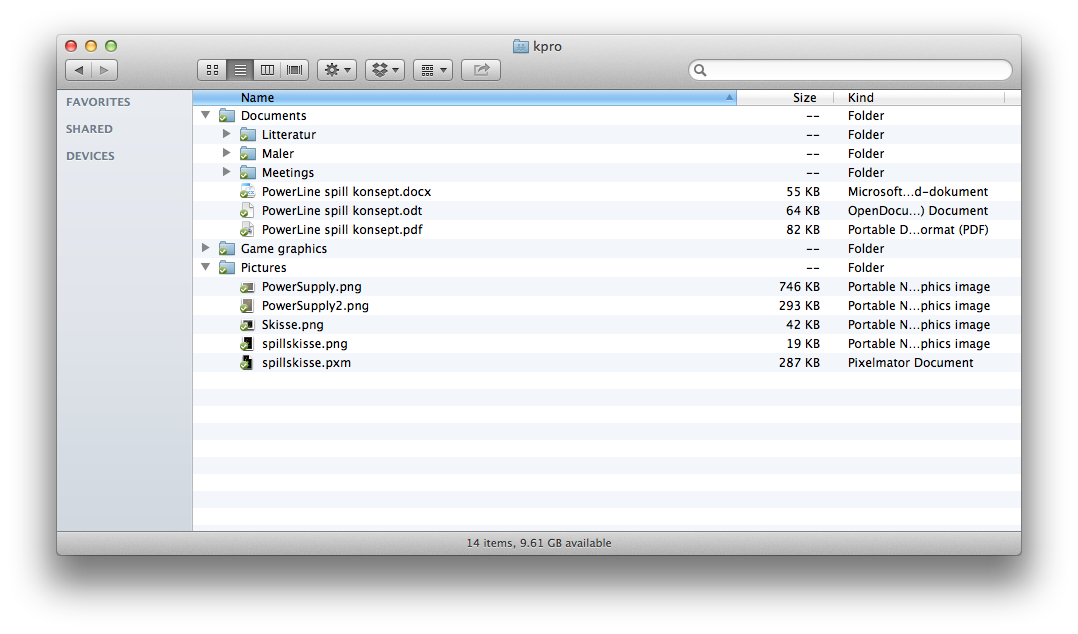
\includegraphics[width=1\textwidth]{pictures/dropbox.png}
      \caption{A shared Dropbox directory}
    \end{figure}
